\documentclass[12pt,letterpaper]{article}
\usepackage[latin1]{inputenc}
\usepackage[spanish]{babel}
\usepackage{amsmath}
\usepackage{amsfonts}
\usepackage{amssymb}
\usepackage{graphicx}
\usepackage[hidelinks]{hyperref}
\usepackage{color}
\graphicspath{{Imagenes/}}
\usepackage[left=2cm,right=2cm,top=2cm,bottom=2cm]{geometry}
\author{Cruz Cervantes Oscar}
\title{EV 2.5 Arreglos de amplificadores de potencia}
\date{08 de Octubre del 2019}
\begin{document}

\begin{center}
\textbf{\huge{Universidad Politecnica de la Zona \\[0.5cm] Metropolitana de Guadalajara }}
\end{center}

\begin{center}

\includegraphics[width=0.65\textwidth]{Imagenes/UPCDLZMDG5783-logo.png}\\[2cm] 
\end{center}
\vspace{0.1cm}
{\large\textbf{Evidencia:} 2.5 Arreglos de amplificadores de potencia\\[0.2cm]\textbf{Alumno:} Cruz Cervantes Oscar\\[0.2cm]\textbf{Profesor:}Mor�n Garabito Carlos Enrique\\[0.2cm]\textbf{Carrera:} Ing.Mecatronica\\[0.2cm]\textbf{Grupo:} 4�B\\[0.2cm]\textbf{Fecha de entrega:} 8 de Octubre del 2019\\[0.2cm]}\\

\vspace{10cm}
\textbf{2.5 Arreglos de amplificadores de potencia}\\[0.3cm]
\textbf{Objetivo:}\\[0.2cm]
Calcular y comprobar la ganancia en voltaje de un Amplificador Operacional inversor, no inversor, sumador, restador, sumador-restador,DAC y ADC por medio de simulaciones.\\[0.5cm]
\vspace{0.2cm}
\textbf{Materiales:}
\begin{itemize}
\item Calculadora
\item Programador Orcad
\item Programador Proteus
\item Impresiones de ejercicios
\end{itemize}
\vspace{0.2cm}
\textbf{Procedimiento:}\\[0.2cm]

El amplificador operacional inversor\\[0.2cm]
1.1 Represente en el simulador el circuito de la figura 1 utilizando los siguientes valores:
\begin{itemize}
\item $R2=10k\Omega$
\item $R1=1k\Omega$
\item Un amplificador LM741 
\item Un voltaje de 250mV
\item Una polaridad de +15 -15 con un 1KHz
\end{itemize}

\begin{figure}[h]
\begin{center}
\centering
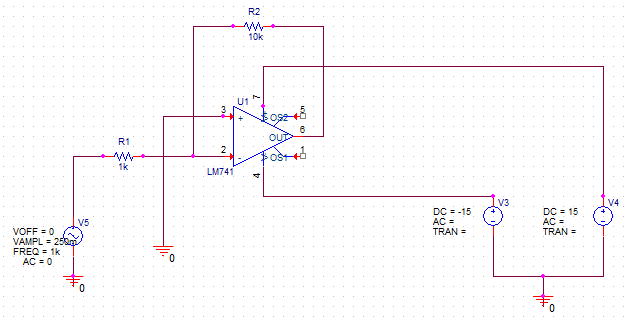
\includegraphics[width=0.50\textwidth]{Imagenes/Captura_1.PNG} 
\caption{Amplificador operacional inversor}
\end{center}
\end{figure}
\vspace{10cm}
1.2 Anota los siguientes resultados la ganancia y amplificaci�n de la simulaci�n junto con su grafica correspondiente que se muestra en la figura 2.\\
 \begin{figure}[h]
\begin{center}
\centering
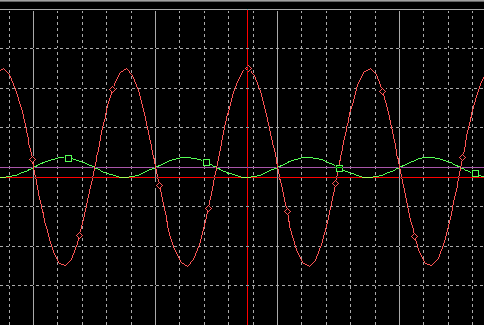
\includegraphics[width=0.50\textwidth]{Imagenes/Captura_2.PNG} 
\caption{Ondas de un amplificador operacional inversor}
\end{center}
\end{figure}

\textbf{Ganancia}\\[0.2cm]
$-(R2 \div R1)=10$\\[0.2cm]
\textbf{Amplificaci�n Entrada y Salida}\\[0.2cm]
$Vi=250mV\approx249.948mV$\\[0.2cm]
$(Vi)(R2 \div R1)=2500mV\approx2499mV$\\[0.2cm]

1.3 Realiza nuevamente los pasos del punto 1.2 asignando los siguientes valores $R2=2.2k\Omega$ y $R1=1k\Omega$ (realiza el siguiente circuito de la figura 3)\\[0.2cm]

\begin{figure}[h]
\begin{center}
\centering
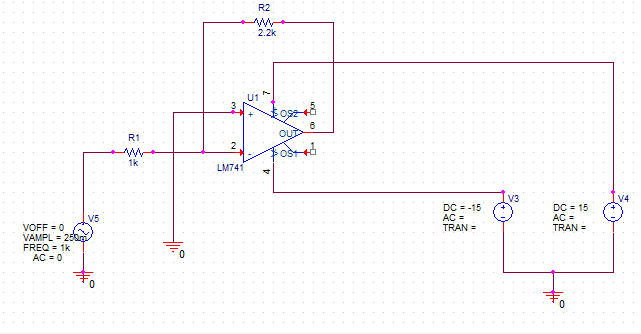
\includegraphics[width=0.50\textwidth]{Imagenes/Captura_3.PNG} 
\caption{Amplificador operacional inversor}
\end{center}
\end{figure}
Se muestra la siguiente grafica de la figura 4 en el que se muestra la amplificacion de entrada y salida de la figura 3.\\[1cm]
 \begin{figure}[h]
\begin{center}
\centering
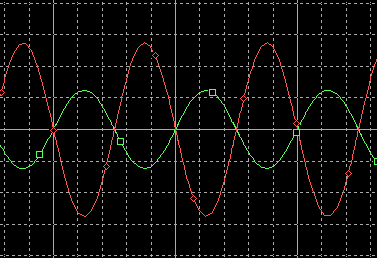
\includegraphics[width=0.50\textwidth]{Imagenes/Captura_4.PNG} 
\caption{Ondas de un amplificador operacional inversor}
\end{center}
\end{figure}
\\[0.1cm]
\textbf{Ganancia}\\[0.2cm]
$-(R2 \div R1)=2.2$\\[0.2cm]
\textbf{Amplificaci�n Entrada y Salida}\\[0.2cm]
$Vi=250mV\approx249.970mV$\\[0.2cm]
$(Vi)(R2 \div R1)=500mV\approx550.11mV$\\[0.2cm]
1.4 Responde las siguientes preguntas despues de realizar las anteriores simulaciones.

\begin{itemize}
\item \textbf{�Son iguales los resultados para la simulacion y la medicion? Explica brevemente sus observaciones.}\\[0.1cm]
En este caso entre una simulacion y una medicion siempre debe de haber una diferencia minima de decimales ya que no siempre son exactas las medidas.
\item \textbf{�El error(porcentaje) encontrado en las simulaciones y en las mediciones con respecto a los calculos teoricos se encuentra dentro la tolerancia dada por el curso?}\\[0.1cm]
Si
\item \textbf{�Encontro alguna relacion entre los resultados y la hipotesis propuesta en las consideraciones teoricas de este proyecto?Explique brevemente.}\\[0.1cm]
La diferencia de error que hay entre V1 y V0 del amplificador.
\item \textbf{�En que forma afecta al funcionamiento del Op Amp la frecuencia de la se�al de entrada?}\\[0.1cm]
Entre mayor frecuencia de operacionmenor sera la ganancia (ancho de banda).
\item \textbf{�Cual es el valor maximo de voltaje de entrada que podria operar confiablemente el amplificador inversor utilicado en este proyecto ?Explique brevemente}\\[0.1cm]
En un LM741 con -/+15v, la oscilacion de la entrada en modo comun deberia estar dentro de +/-12v. Los voltajes arriba de 15v pueden da�ar el Op Amp independientemente del voltaje de la fuente.
\item \textbf{�Cual es la frecuencia maxima y minima que es capaz de operar el Op Amp utilizado en esta practica?}\\[0.1cm]
De 100kHz a un millon, pero eso afectaria la ganancia dandonos resultados erroneos.
\item \textbf{�Que sucederia si el Op Amp utilizado se polariza con +/-12v en lugar de +/-15v?}\\[0.1cm]
No afecta mucho ya que esta dentro del rango de voltaje.
\item \textbf{�Se logro comprobar la hipotesis propuesta para este proyecto?}\\[0.1cm]
Si, ya que a base de investigacion y calculos se pudo comprobar que en un Op Amp siempre hay un offset una diferencia entre V1-Vn.

\end{itemize}

El amplificador operacional no inversor\\[0.2cm]

2.1 Represente en el simulador el circuito de la figura 5 utilizando los siguientes valores:
\begin{itemize}
\item $R2=10k\Omega$
\item $R1=1k\Omega$
\item Un amplificador LM741 
\item Un voltaje de 250mV
\item Una polaridad de +15 -15 con un 1KHz
\end{itemize}

\begin{figure}[h]
\begin{center}
\centering
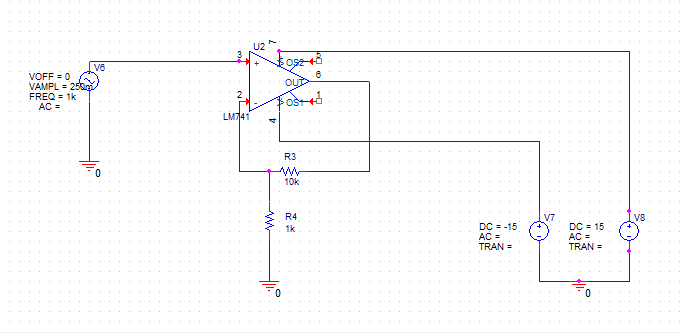
\includegraphics[width=0.50\textwidth]{Imagenes/Captura_5.PNG} 
\caption{Amplificador operacional no inversor}
\end{center}
\end{figure}
\vspace{10cm}
2.2 Anota los siguientes resultados la ganancia y amplificaci�n de la simulaci�n junto con su grafica correspondiente que se muestra en la figura 5.\\
\begin{figure}[h]
\begin{center}
\centering
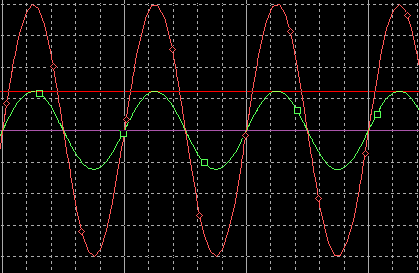
\includegraphics[width=0.50\textwidth]{Imagenes/Captura_6.PNG} 
\caption{Ondas de un amplificador operacional no inversor}
\end{center}
\end{figure}

\textbf{Ganancia}\\[0.2cm]
$1+(R2 \div R1)=11$\\[0.2cm]
\textbf{Amplificaci�n Entrada y Salida}\\[0.2cm]
$Vi=250mV\approx249.948mV$\\[0.2cm]
$(Vi)(1+(R2 \div R1))=2.75mV\approx2.7339mV$\\[0.2cm]

2.3 Realiza nuevamente los pasos del punto 1.2 asignando los siguientes valores $R2=2.2k\Omega$ y $R1=1k\Omega$ (realiza el siguiente circuito de la figura 7)\\[0.2cm]

\begin{figure}[h]
\begin{center}
\centering
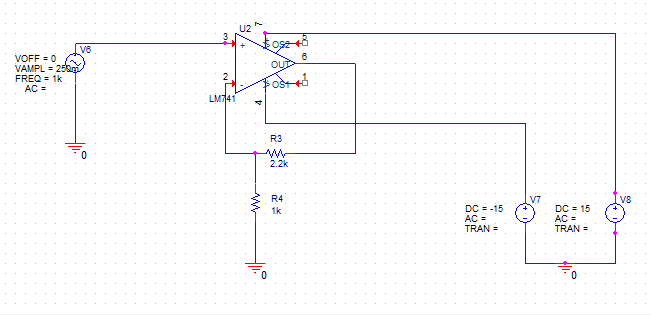
\includegraphics[width=0.50\textwidth]{Imagenes/Captura_7.PNG} 
\caption{Amplificador operacional no inversor}
\end{center}
\end{figure}
Se muestra la siguiente grafica de la figura 8 en el que se muestra la amplificacion de entrada y salida de la figura 7.\\[1cm]
\begin{figure}[h]
\begin{center}
\centering
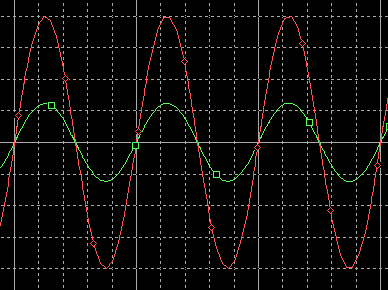
\includegraphics[width=0.50\textwidth]{Imagenes/Captura_8.PNG} 
\caption{Ondas de un amplificador operacional no inversor}
\end{center}
\end{figure}
\\[0.1cm]
\textbf{Ganancia}\\[0.2cm]
$1+(R2 \div R1)=3.2$\\[0.2cm]
\textbf{Amplificaci�n Entrada y Salida}\\[0.2cm]
$Vi=250mV\approx249.970mV$\\[0.2cm]
$(Vi)(1+(R2 \div R1))=800mV\approx792mV$\\[0.2cm]
1.4 Responde las siguientes preguntas despues de realizar las anteriores simulaciones.

\begin{itemize}
\item \textbf{�Son iguales los resultados para la simulacion y la medicion? Explica brevemente sus observaciones.}\\[0.1cm]
En este caso entre una simulacion y una medicion siempre debe de haber una diferencia minima de decimales ya que no siempre son exactas las medidas.
\item \textbf{�Encuentra alguna relacion entre los resultados obtenidos y las lineas de accion propuestas en las consideraciones teoricas de esta practica?Explique.}\\[0.1cm]
No, ya que hay cierta variabilidad entre los resultados de las simulaciones a lo teorico.
\item \textbf{�En que forma afecta la frecuencia de la se�al de entrada al funcionamiento del Op Amp?}\\[0.1cm]
Entre mayor frecuencia de operacion menor sera la ganancia (ancho de banda).
\item \textbf{�Cual es el valor maximo de voltaje de entrada con el que podria operar confiablemente el amplificador no inversor utilizado en este proyecto ?Explique}\\[0.1cm]
En este caso que es un LM741 con -/+15v.
\item \textbf{�Cual son las frecuencias maxima y minima que es capaz de operar el Op Amp utilizado en esta practica?}\\[0.1cm]
De 100kHz, pero eso afectaria la ganancia dandonos resultados erroneos.
\item \textbf{�Que sucederia si el Op Amp utilizado se polariza con +/-12v en lugar de +/-15v?}\\[0.1cm]
No afecta mucho ya que esta dentro del rango de voltaje.
\item \textbf{�Que diferencia encuentra entre el Op Amp no inversor y el Op Amp inversor?}\\[0.1cm]
Las ondas que emiten en el osciloscopio son diferentes la del no inversor van del mismo lado y del inversor van del lado contrario.
\item \textbf{�Se pudo comprobar la hipotesis propuesta para este proyecto?}\\[0.1cm]
Si, ya que a base de investigacion y calculos se pudo comprobar que en un Op Amp siempre tiene una diferencia entre las ondas.
\end{itemize}



Sumador con Op Amp\\[0.2cm]

3.1 Represente en el simulador el circuito de la figura 9 utilizando los siguientes valores:
\begin{itemize}
\item $R5=10k\Omega$
\item $R7=1.5k\Omega$
\item $R6=1k\Omega$
\item $R8=590\Omega$
\item Un amplificador LM741 
\item Un voltaje de 300mV
\item Una polaridad de +15 -15 con un 1KHz
\end{itemize}

\begin{figure}[h]
\begin{center}
\centering
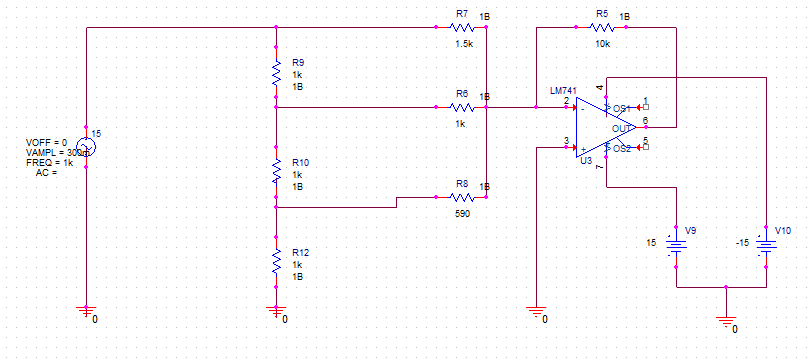
\includegraphics[width=0.50\textwidth]{Imagenes/Captura_9.PNG} 
\caption{Sumador Op Amp}
\end{center}
\end{figure}
\vspace{10cm}
3.2 Mida en el osciloscopio virtual el voltaje para cada entrada del sumador como en la figura 10.\\
\begin{figure}[h]
\begin{center}
\centering
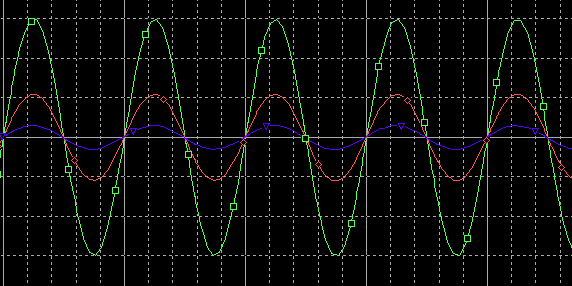
\includegraphics[width=0.50\textwidth]{Imagenes/Captura_10.PNG} 
\caption{Ondas de un amplificador operacional sumador}
\end{center}
\end{figure}

\textbf{Voltaje}\\[0.2cm]
VR7 = 296.321mv \\[0.2cm]
VR6 =108.652mv\\[0.2cm]
VR8 = 29.477mv\\[0.2cm]

3.3 Ahora mostrar los resultados de entrada y salida del sumandor por medio del osciloscopio como se muestra en la figura 11)\\[0.2cm]

\begin{figure}[h]
\begin{center}
\centering
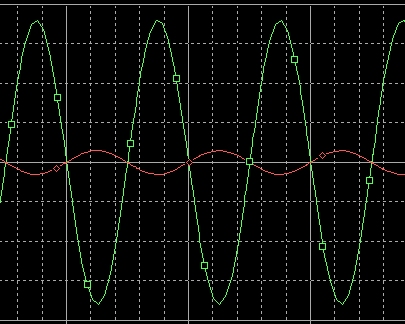
\includegraphics[width=0.50\textwidth]{Imagenes/Captura_11.PNG} 
\caption{Ondas de Amplificador operacional sumador Salida-Entrada}
\end{center}
\end{figure}
\vspace{10cm}
\textbf{Voltaje Salida-Entrada}\\[0.2cm]
Vin = 300mv \\[0.2cm]
V0 =3.57\\[0.2cm]


Restador con Op Amp\\[0.2cm]

4.1 Represente en el simulador el circuito de la figura 11 utilizando los siguientes valores:
\begin{itemize}
\item $R13=40k\Omega$
\item $R14=2k\Omega$
\item $R15=4k\Omega$
\item $R16=120k\Omega$
\item Un amplificador LM741 
\item Un voltaje de 300mV
\item Una polaridad de +15 -15 con un 1KHz
\end{itemize}

\begin{figure}[h]
\begin{center}
\centering
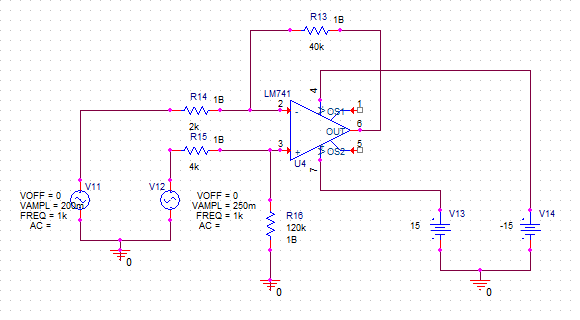
\includegraphics[width=0.50\textwidth]{Imagenes/Captura_12.PNG} 
\caption{Restador Op Amp}
\end{center}
\end{figure}
\vspace{10cm}
4.2 Mida en el osciloscopio virtual el voltaje para cada entrada del restador como en la figura 13.\\
\begin{figure}[h]
\begin{center}
\centering
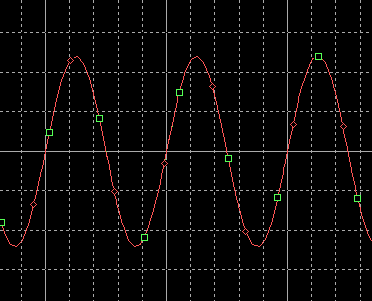
\includegraphics[width=0.50\textwidth]{Imagenes/Captura_13.PNG} 
\caption{Ondas de un amplificador operacional restador}
\end{center}
\end{figure}

\textbf{Voltaje}\\[0.2cm]
VR14 = 239.035mv \\[0.2cm]
VR15 =239.035mv\\[0.2cm]


4.3 Ahora mostrar los resultados de entrada y salida del restador por medio del osciloscopio como se muestra en la figura 14)\\[0.2cm]

\begin{figure}[h]
\begin{center}
\centering
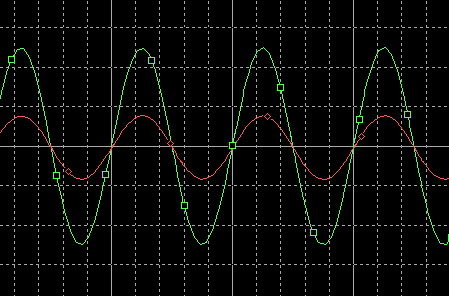
\includegraphics[width=0.50\textwidth]{Imagenes/Captura_14.PNG} 
\caption{Ondas de Amplificador operacional restador Salida-Entrada}
\end{center}
\end{figure}
\vspace{10cm}
\textbf{Voltaje Salida-Entrada}\\[0.2cm]
Vin = 200mv \\[0.2cm]
V0 =76.7\\[0.2cm]



Sumador - Restador con Op Amp\\[0.2cm]

5.1 Represente en el simulador el circuito de la figura 15 

\begin{figure}[h]
\begin{center}
\centering
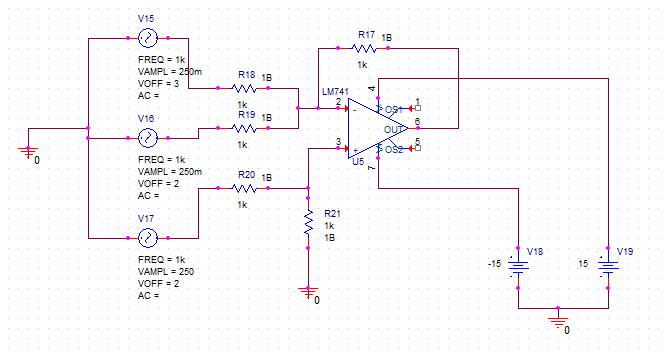
\includegraphics[width=0.50\textwidth]{Imagenes/Captura_15.PNG} 
\caption{Sumador - Restador Op Amp}
\end{center}
\end{figure}
\vspace{10cm}
5.2 Mida en el osciloscopio virtual el voltaje para cada entrada del sumador - restador como en la figura 16.\\
\begin{figure}[h]
\begin{center}
\centering
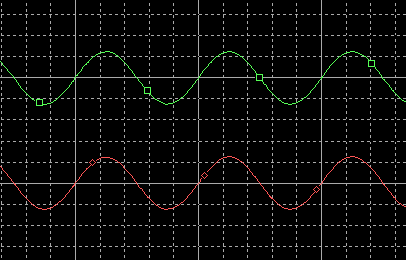
\includegraphics[width=0.50\textwidth]{Imagenes/Captura_16.PNG} 
\caption{Ondas de un amplificador operacional restador}
\end{center}
\end{figure}

\textbf{Voltaje}\\[0.2cm]
VR18 = 2 \\[0.2cm]
VR19 =3\\[0.2cm]


5.3 Ahora mostrar los resultados de salida del sumador - restador por medio del osciloscopio como se muestra en la figura 17)\\[0.2cm]

\begin{figure}[h]
\begin{center}
\centering
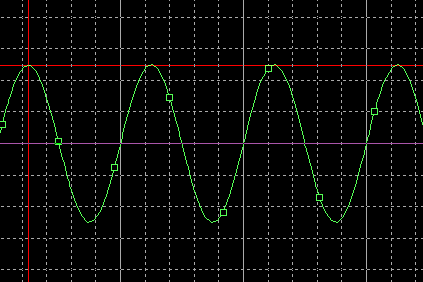
\includegraphics[width=0.50\textwidth]{Imagenes/Captura_17.PNG} 
\caption{Ondas de Amplificador operacional sumador - restador Salida}
\end{center}
\end{figure}
\vspace{10cm}
\textbf{Voltaje Salida}\\[0.2cm]
V0 =-250mV\\[0.2cm]





El amplificador operacional inversor\\[0.2cm]
6.1 Represente en el simulador el circuito de la figura 1 utilizando los siguientes valores:
\begin{itemize}
\item $R2=100k\Omega$
\item $R1=1.2k\Omega$
\item Un amplificador LM741 
\item Un voltaje de 12mV
\item Una polaridad de +15 -15 con un 1KHz
\end{itemize}

\begin{figure}[h]
\begin{center}
\centering
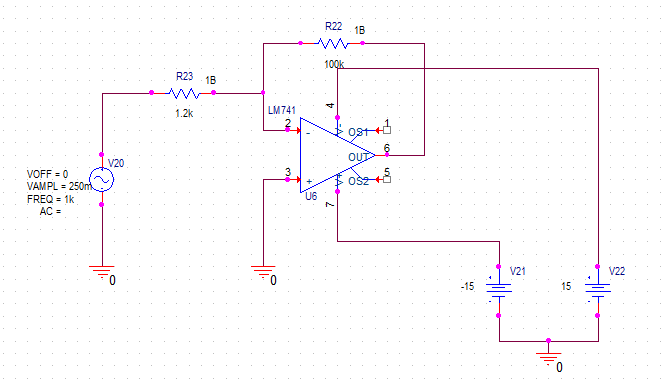
\includegraphics[width=0.50\textwidth]{Imagenes/Captura_18.PNG} 
\caption{Amplificador operacional inversor}
\end{center}
\end{figure}
\vspace{10cm}
6.2 Anota los siguientes resultados la ganancia y amplificaci�n de la simulaci�n junto con su grafica correspondiente que se muestra en la figura 19.\\
 \begin{figure}[h]
\begin{center}
\centering
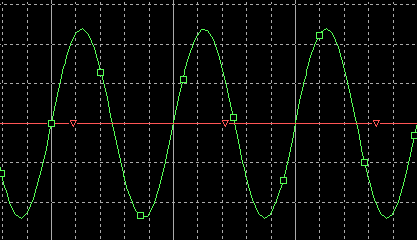
\includegraphics[width=0.50\textwidth]{Imagenes/Captura_19.PNG} 
\caption{Ondas de un amplificador operacional inversor}
\end{center}
\end{figure}

\textbf{Ganancia}\\[0.2cm]
$-(R2 \div R1)=10$\\[0.2cm]
\textbf{Amplificaci�n Entrada y Salida}\\[0.2cm]
$Vi=12mV\approx12mV$\\[0.2cm]
$(Vi)(R2 \div R1)=1mV\approx1mV$\\[0.2cm]








El amplificador operacional no inversor\\[0.2cm]

7.1 Represente en el simulador el circuito de la figura 20 utilizando los siguientes valores:
\begin{itemize}
\item $R2=300k\Omega$
\item $R1=1.5k\Omega$
\item Un amplificador LM741 
\item Un voltaje de 15mV
\item Una polaridad de +15 -15 con un 1KHz
\end{itemize}

\begin{figure}[h]
\begin{center}
\centering
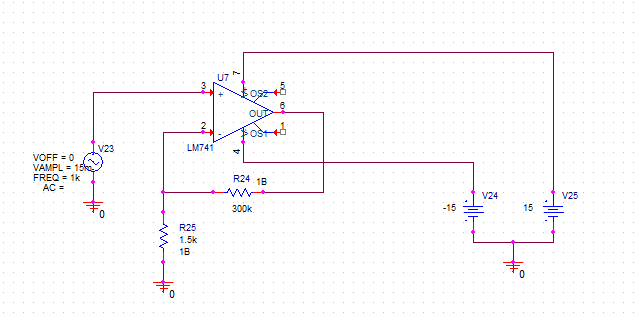
\includegraphics[width=0.50\textwidth]{Imagenes/Captura_21.PNG} 
\caption{Amplificador operacional no inversor}
\end{center}
\end{figure}
\vspace{10cm}
7.2 Anota los siguientes resultados la ganancia y amplificaci�n de la simulaci�n junto con su grafica correspondiente que se muestra en la figura 21.\\
\begin{figure}[h]
\begin{center}
\centering
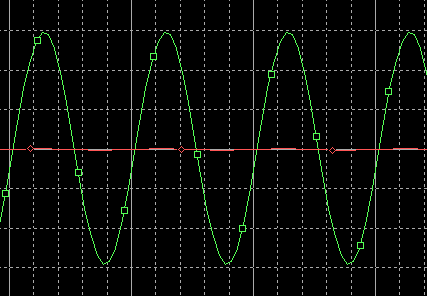
\includegraphics[width=0.50\textwidth]{Imagenes/Captura_20.PNG} 
\caption{Ondas de un amplificador operacional no inversor}
\end{center}
\end{figure}

\textbf{Ganancia}\\[0.2cm]
$1+(R2 \div R1)=21$\\[0.2cm]
\textbf{Amplificaci�n Entrada y Salida}\\[0.2cm]
$Vi=15mV\approx15mV$\\[0.2cm]
$(Vi)(1+(R2 \div R1))=3mV\approx3mV$\\[0.2cm]

\vspace{10cm}
\textbf{ADC}
\begin{figure}[h]
\begin{center}
\centering
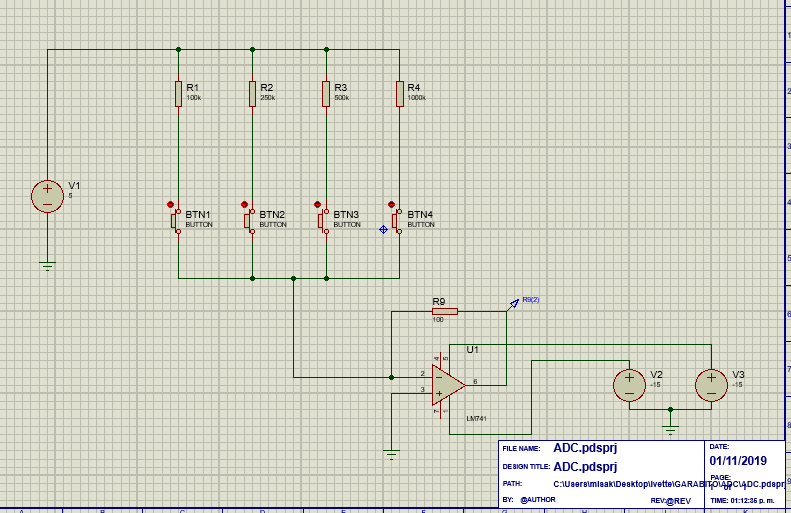
\includegraphics[width=0.50\textwidth]{Imagenes/Captura_24.PNG} 
\caption{ADC}
\end{center}
\end{figure} 

\begin{figure}[h]
\begin{center}
\centering
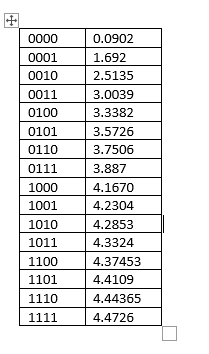
\includegraphics[width=0.50\textwidth]{Imagenes/Captura_241.PNG} 
\caption{ADC}
\end{center}
\end{figure} 

\textbf{DAC}
\begin{figure}[h]
\begin{center}
\centering
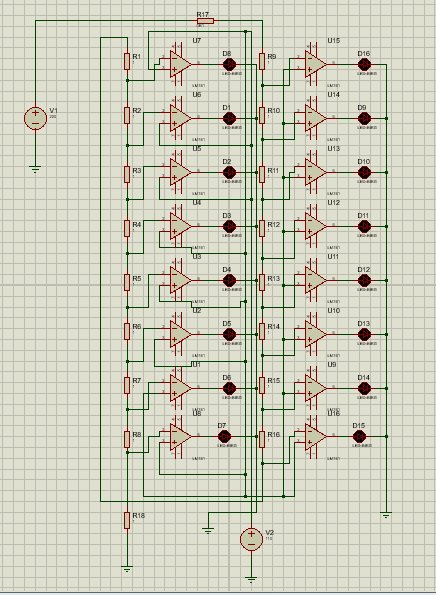
\includegraphics[width=0.50\textwidth]{Imagenes/Captura_23.PNG} 
\caption{DAC}
\end{center}
\end{figure} 

\begin{figure}[h]
\begin{center}
\centering
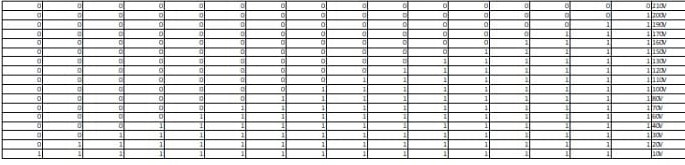
\includegraphics[width=0.50\textwidth]{Imagenes/Captura_231} 
\caption{DAC}
\end{center}
\end{figure} 

\textbf{\large{Bibliograf�as}}\
\begin{center}
\emph{Creative Commons BY NC SA. (2013). INEVITABLE.eu. Obtenido de La electronica simple y clara.} Obtenido de: \textcolor{blue}{ http://www1.frm.utn.edu.ar/medidase2/tp/tp6.pdf}\\[0.3cm]
\end{center}
\end{document}